\documentclass{article}
\usepackage{amsmath}
\usepackage{amsfonts}
\usepackage{amssymb}
\usepackage{graphicx}
\usepackage{listings}
\usepackage{color}
\usepackage{hyperref}
\usepackage[a4paper, margin=1in]{geometry}

\definecolor{mygreen}{rgb}{0,0.6,0}
\definecolor{mygray}{rgb}{0.5,0.5,0.5}
\definecolor{mymauve}{rgb}{0.58,0,0.82}

\lstset{ %
  backgroundcolor=\color{white},   
  basicstyle=\footnotesize,        
  breaklines=true,                 
  captionpos=b,                    
  commentstyle=\color{mygreen},    
  escapeinside={\%*}{*)},          
  keywordstyle=\color{blue},       
  stringstyle=\color{mymauve},     
}

\begin{document}

\textbf{1 (Problema de apilamiento de libros)} Aquí hay una situación física interesante en la que aparece la Serie Armónica. El problema fue publicado por Paul Johnson en 1955 \cite{101}. El código \texttt{harmonic.ipynb} puede ser útil en esta pregunta.

Deseo crear una torre inclinada de libros utilizando múltiples copias idénticas de un libro. Usando \(n\) libros organizados en una torre perpendicular al borde de la mesa, empujo el libro superior tan lejos como puedo, y hago lo mismo con el siguiente libro abajo, trabajando hacia la base de la torre. Ver la figura abajo cuando \(n = 4\). Podemos asumir que los libros y la mesa son lo suficientemente rígidos como para que no haya movimientos verticales.

\begin{figure}[h]
    \centering
    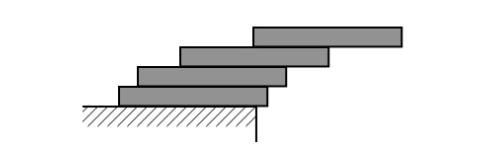
\includegraphics[width=0.7\textwidth]{pictures/block.png}
    \label{fig:1img}
\end{figure}

\begin{itemize}
    \item[(a)] Demuestra que utilizando \(n\) libros, el voladizo (en unidades de libros) se puede escribir como la Serie Armónica
    \[
    \frac{1}{2} \left(1 + \frac{1}{2} + \frac{1}{3} + \cdots + \frac{1}{n}\right).
    \]
    Deduce que usando 4 libros, el voladizo excede la longitud de un libro.
    
    \item[(b)] Grafica el voladizo (en unidades de libros) en función del número de libros usados para construir la torre. Considera hasta 1000 libros. Sugerencia: usa escala logarítmica en el eje horizontal.
    
    \item[(c)] En la misma gráfica, traza el resultado cuando se usa la ecuación 1.4 (aproximación logarítmica de la Serie Armónica) para calcular el voladizo.
    
    \item[(d)] Usando la aproximación logarítmica:
    \begin{itemize}
        \item[(i)] estima el voladizo cuando se usan \(10^6\) libros para crear la torre. (Respuesta: voladizo de alrededor de 7 libros de longitud.)
        
        \item[(ii)] estima el número de libros necesarios para construir una torre inclinada con un voladizo de 10 libros de longitud. (Tu respuesta probablemente sea mayor que el número estimado de libros físicos que existen en el mundo.)
    \end{itemize}
\end{itemize}

\textbf{2 (Aproximaciones famosas para \(\pi\))} A continuación se presentan tres aproximaciones históricamente importantes para \(\pi\).

\begin{itemize}
    \item \textbf{Serie de Madhava} (siglo XIV), a veces llamada la \textit{aproximación de Gregory-Leibniz} (1671-1673)
    \[
    \pi = 4 \left( 1 - \frac{1}{3} + \frac{1}{5} - \frac{1}{7} + \cdots \right)
    \]
    
    \item \textbf{Producto de Wallis} (1656)
    \[
    \pi = 2 \left( \frac{2}{1} \cdot \frac{2}{3} \right) \cdot \left( \frac{4}{3} \cdot \frac{4}{5} \right) \cdot \left( \frac{6}{5} \cdot \frac{6}{7} \right) \cdots
    \]
    
    \item \textbf{Fórmula de Viète} (1593)
    \[
    \pi = 2 \cdot \frac{2}{\sqrt{2}} \cdot \frac{2}{\sqrt{2 + \sqrt{2}}} \cdot \frac{2}{\sqrt{2 + \sqrt{2 + \sqrt{2}}}} \cdots
    \]
\end{itemize}

Sea \(n\) el número de iteraciones en cada esquema de aproximación. Por ejemplo, la iteración cero (\(n = 0\)) da 4, 2 y 2 para las tres aproximaciones respectivamente.

\begin{itemize}
    \item[(a)] En el mismo conjunto de ejes, grafica los resultados de las tres aproximaciones en función del número de iteraciones hasta \(n = 10\).
    
    \item[(b)] En un conjunto de ejes logarítmicos, grafica el error fraccional absoluto
    \[
    \left| \frac{\text{Estimación después de } n \text{ iteraciones} - \pi}{\pi} \right|
    \]
    para las tres aproximaciones hasta \(n = 100\). Esto nos da una idea de qué tan rápido las aproximaciones convergen a \(\pi\).
    
    Deberías encontrar que el error para la fórmula de Viète no parece disminuir por debajo de un límite mínimo de alrededor de \(10^{-16}\). La razón de esto es el \textit{epsilon de máquina}, que será discutido en la sección \(\S 2.2\).
    
    \item[(c)] Recuerda que una estimación \(x\) de \(\pi\) es precisa hasta \(p\) lugares decimales si \(\left| x - \pi \right| < 0.5 \times 10^{-p}\). Para cada una de las tres aproximaciones de \(\pi\), calcula cuántas iteraciones se necesitan para obtener \(\pi\) preciso hasta 5 lugares decimales. (Respuestas: 200000, 157080 y 9.)
\end{itemize}

\textbf{3 (Fórmula de Ramanujan para \(\pi\))} En 1910, Ramanujan dio la siguiente fórmula para \(\pi\).

\[
\pi = \left[ \frac{2\sqrt{2}}{9801} \sum_{n=0}^{\infty} \frac{(4n)!(1103 + 26390n)}{(n!)^4 396^{4n}} \right]^{-1}.
\]

(Famosamente, él simplemente "escribió" muchas de estas fórmulas.) Calcula las primeras 3 iteraciones de esta aproximación. ¿A cuántos lugares decimales es precisa cada una de estas aproximaciones? Intenta escribir un código que calcule la serie hasta \(n\) términos. ¿Puede tu código evaluar el resultado con precisión, por ejemplo, cuando \(n = 10\)? Si no, explica por qué.


\textbf{4 (Número recíproco de Fibonacci)} Usa \texttt{fibonacci.ipynb} como punto de partida.

La constante recíproca de Fibonacci está dada por

\[
\psi = \sum_{n=1}^{\infty} \frac{1}{F_n} = 3.35988566624317755\ldots
\]

\begin{itemize}
    \item[(a)] Calcula la suma hasta 20 términos.  
    Sugerencia: Intenta hacer esto de manera vectorizada usando arreglos en lugar de un bucle.
    
    \item[(b)] Calcula cuántos términos son necesarios para obtener \(\psi\) con 10 decimales de precisión. (Respuesta: 49.)
\end{itemize}


\textbf{5 (Secuencias generalizadas de Fibonacci)} Usa \texttt{fibonacci.ipynb} como punto de partida.

\begin{itemize}
    \item[(a)] Supongamos que usamos diferentes valores iniciales \(F_0\) y \(F_1\). Usa Python para investigar el comportamiento de la razón \(R_n := \frac{F_n}{F_{n-1}}\). Muestra que \(R_n\) siempre converge al número áureo.  
    (Si te gusta un desafío, podrías demostrar este comportamiento usando deslizadores.)
    
    \item[(b)] (\textit{Secuencias de Lucas}) Sean \(P\) y \(Q\) enteros fijos (no ambos cero). Define la secuencia de Lucas, \(U_n(P, Q)\), por las siguientes reglas:
    \[
    U_0 = 0, \quad U_1 = 1, \quad U_n = PU_{n-1} - QU_{n-2}.
    \]
    
    Nota que la secuencia de Fibonacci corresponde a \(U_n(1, -1)\).  
    Escribe un código que grafique el comportamiento para \(n\) grande de la razón de términos consecutivos \(R_n := \frac{U_{n+1}}{U_n}\) para los siguientes valores de \(P\) y \(Q\):
    \begin{itemize}
        \item[i.] \((P, Q) = (3, 1)\)
        \item[ii.] \((P, Q) = (2, 1)\)
        \item[iii.] \((P, Q) = (1, 1)\)
    \end{itemize}
    
    Haz una conjetura sobre los valores del rango de \(P\) tales que \(R_n\) sea una secuencia convergente.  
    (Respuesta: ver \url{https://mathworld.wolfram.com/LucasSequence.html})
\end{itemize}


\textbf{6 (Orden de convergencia)} Dada una secuencia convergente, es natural preguntar: \textit{¿qué tan rápido converge la secuencia?} En esta pregunta, exploramos cómo cuantificar la velocidad de convergencia.  
Supongamos que una secuencia \((x_n)\) converge a \(x\). Define el error absoluto, \(E_n\), como la secuencia

\[
E_n = |x_n - x|.
\]

La velocidad de convergencia se puede cuantificar mediante dos constantes positivas: la \textit{tasa} (\(C\)) y el \textit{orden} (\(q\)) de convergencia, definido a través de la ecuación

\[
\lim_{n \to \infty} \frac{E_{n+1}}{(E_n)^q} = C > 0.
\]

\begin{itemize}
    \item[(a)] Verifica manualmente que la secuencia \(\left(\frac{1}{n}\right)\) converge con \(q = C = 1\).
    
    \item[(b)] Para la mayoría de las aplicaciones, solo el orden de convergencia es de interés, ya que es un mejor indicador de qué tan rápido converge la secuencia. Se puede demostrar que podemos estimar \(q\) usando la fórmula
    \[
    q \approx \frac{\ln(E_{n+1}/E_n)}{\ln(E_n/E_{n-1})},
    \]
    donde \(n\) debería ser lo suficientemente grande como para que \(q\) se estabilice, pero no tan grande como para que el denominador en la fórmula sea cero.
    
    \begin{itemize}
        \item[i.] Usando esta aproximación, verifica (usando Python) que la razón de números de Fibonacci \(R_n = \frac{F_{n+1}}{F_n}\) converge con un orden menor que 1.  
        Sugerencia: podría ser útil graficar \(q\) como una función de \(n\). Deberías encontrar que la gráfica se estabiliza en \(q = 1\) antes de volverse indefinida cuando \(n\) es demasiado grande.
        
        \item[ii.] Considera la serie de Madhava para \(\pi\) en la Pregunta 2. Muestra que \(q < 1\).  
        Técnicamente, decimos que la convergencia de la serie es sublineal (es decir, terriblemente lenta).
        
        \item[iii.] Conjetura una secuencia que converge superlinealmente (\(q > 1\)) y demuestra gráficamente esta propiedad.
    \end{itemize}
\end{itemize}

\textbf{7} En \texttt{continuityslider.ipynb} (\(\S 1.7\)), agrega un deslizador en la interfaz gráfica de usuario (GUI) para que el valor de \(x_0\) se pueda cambiar.

\textbf{8 (El huerto de Euclides)} La función de Thomae (\(\S 1.8\)) tiene una conexión interesante con el siguiente problema, a veces llamado el huerto de Euclides o el problema de los puntos visibles.

Considera puntos de una cuadrícula con coordenadas enteras positivas \((m, n)\). Se dice que un punto de la cuadrícula \(P\) es visible desde \((0,0)\) si una línea recta que une \((0,0)\) con \(P\) no pasa a través de ningún otro punto de la cuadrícula. Por ejemplo, como se muestra en la figura de abajo, el punto \((1, 2)\) es visible desde \((0,0)\), pero \((2, 4)\) no lo es.

\begin{figure}[h]
    \centering
    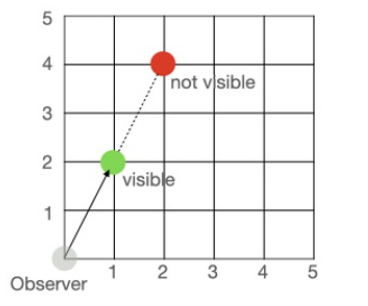
\includegraphics[width=0.7\textwidth]{pictures/visible.png}
    \label{fig:8img}
\end{figure}


Primero deberías intentar experimentar en un trozo de papel cuadriculado para formular una conjetura sobre qué puntos son visibles desde \((0, 0)\).

\begin{itemize}
    \item[(a)] Escribe un código que produzca una cuadrícula y marque con un punto rojo cada punto visible desde \((0,0)\) (deberás imponer un límite razonable).
    
    \item[(b)] Para cada punto visible \((m, n)\), grafica su imagen bajo la siguiente aplicación
    \[
    F(m, n) = \left( \frac{m}{m + n}, \frac{1}{m + n} \right).
    \]
    
    ¿Qué observas? ¿Puedes explicar cómo funciona esta transformación?  
    (Respuesta: ¡Ves la función de Thomae!)
\end{itemize}


\textbf{9 (Búsqueda de raíces)} Usa el código de bisección para resolver los siguientes problemas. Da tus respuestas con 4 decimales.

\begin{itemize}
    \item[(a)] Resuelve la ecuación \(x^3 - x^2 - x - 1 = 0\).  
    Sugerencia: Comienza graficando.
    
    \item[(b)] Resuelve \(\frac{\sin x}{x} = 0.9\) (verificando así el punto de intersección visto en la fig. 1.8).
    
    \item[(c)] Encuentra el valor numérico de \(\sqrt{3}\) usando solo las cuatro operaciones básicas \(+\), \(-\), \(\times\), \(\div\).  
    Sugerencia: Comienza definiendo \(f(x) = x^2 - 3\).
\end{itemize}

\textbf{10 (Razón Áurea Generalizada)} Supongamos que generalizamos la Razón Áurea a \(\phi_n\), definida como la raíz positiva del siguiente polinomio de orden \(n\)

\[
x^n - x^{n-1} - x^{n-2} - \dots - 1 = 0.
\]

Por ejemplo, \(\phi_1 = 1\) y \(\phi_2 = 1.618\).  
Escribe un código que grafique la secuencia \(\phi_n\) (obtenida mediante bisección). Haz una conjetura sobre el valor de \(\lim_{n \to \infty} \phi_n\).

\textbf{11 (Método de Newton-Raphson)} Sea \(f\) una función diferenciable en \(\mathbb{R}\). El método de Newton-Raphson para encontrar la raíz de la ecuación \(f(x) = 0\) comprende los siguientes pasos.

\begin{itemize}
    \item Comienza con una suposición inicial \(x_0\).
    \item Calcula
    \[
    x_{n+1} = x_n - \frac{f(x_n)}{f'(x_n)},
    \]
    donde la expresión para \(f'(x)\) debe ser conocida explícitamente.
    \item Repite la iteración anterior mientras \(|x_{n+1} - x_n| < \epsilon\) para una tolerancia fija \(\epsilon\) especificada por el usuario (por ejemplo, \(0.5 \times 10^{-p}\) para una precisión de \(p\) decimales). Este paso asegura que solo detengamos el proceso cuando los primeros \(p\) decimales estén estabilizados.
\end{itemize}

\begin{itemize}
    \item[(a)] Escribe un código en Python para este método y úsalo para resolver los problemas de la pregunta 9.
    
    \item[(b)] Sea \(x_n\) la estimación de la solución de \(f(x) = x^2 - 3\) después de \(n\) iteraciones usando el método de Newton-Raphson.  
    Calcula el error absoluto \(E_n = |x_n - \sqrt{3}|\) y verifica que el método de Newton-Raphson tiene orden 2. Haz esto calculando \(q\) definido en la pregunta 6.
\end{itemize}

\textbf{12 (Creando una gráfica bonita)} Grafica la función \textit{sinc} \(f : [0, 2\pi] \to \mathbb{R}\) definida por

\[
f(x) = 
\begin{cases} 
\frac{\sin x}{x} & \text{si } x \neq 0, \\
1 & \text{si } x = 0.
\end{cases}
\]

En el mismo conjunto de ejes, grafica su primera y segunda derivada, estimadas usando el método de Euler hacia adelante (es decir, no diferencies nada a mano en esta pregunta). Intenta usar diferentes tipos de líneas en tu gráfica (piensa en los lectores daltónicos). Aquí tienes un ejemplo de salida.

\begin{figure}[h]
    \centering
    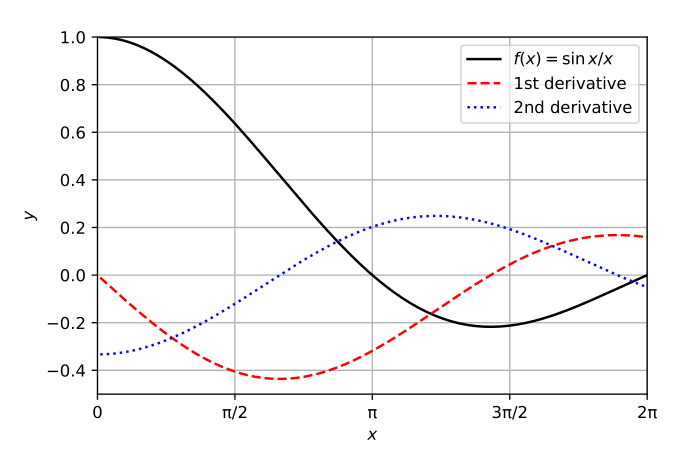
\includegraphics[width=0.7\textwidth]{pictures/sinc.png}
    \caption{Una bonita gráfica de la función \textit{sinc} y sus primeras y segundas derivadas.}
    \label{fig:sinc_derivadas}
\end{figure}


\textbf{13 (Teorema del Valor Medio)} Considera la función \textit{sinc} \(f\) definida en la pregunta anterior. Apliquemos el Teorema del Valor Medio (teorema 1.11) a \(f\) en el intervalo \([0, \pi]\). En particular, determinemos el(los) valor(es) de \(c\) en la declaración del teorema. En otras palabras, deseamos encontrar \(c \in [0, \pi]\) tal que

\[
f'(c) = \frac{f(\pi) - f(0)}{\pi}.
\]

\begin{itemize}
    \item[(a)] Demuestra (a mano) que una solución es \(c = \pi\).
    
    \item[(b)] Usa un algoritmo de búsqueda de raíces para encontrar otra solución con 4 decimales.  
    Tu respuesta debe ser consistente con la línea discontinua en la fig. 1.16 anterior.
\end{itemize}

\textbf{14 (Otro contraejemplo)} Aquí hay otro ejemplo interesante e intuitivo en el análisis. Usa \texttt{counterexample.ipynb} como plantilla.

Considera la función \(f : [0, 1] \to \mathbb{R}\) definida por

\[
f(x) = 
\begin{cases} 
x \left( 2 - \cos \ln x - \sin \ln x \right) & \text{si } x \in (0, 1], \\
0 & \text{si } x = 0.
\end{cases}
\]

Se puede demostrar que \(f\) es estrictamente creciente, sin embargo, hay infinitos puntos donde \(f'(x) = 0\) en \((0, 1]\).

\begin{itemize}
    \item[(a)] Usa Python para graficar la función. Tu gráfica debe demostrar la estructura autosemejante cuando hacemos zoom hacia el origen.
    
    \item[(b)] Demuestra (a mano) que hay puntos de inflexión en \(x = e^{-2n\pi}\) donde \(n \in \mathbb{N}\). Indícalos en tu gráfica.
\end{itemize}


\end{document}